\chapter{Introduction}
\label{sec:introduction}
%\chapter{Einleitung}
%\label{sec:einleitung}

As with many fields in robotics, Human Robot Interaction (HRI) has seen a lot of development in the last twenty years. Research has come from tele-operated assistive robots to dynamically and independently collaborating robots. This advancement is expressed by the newly joined terms and taxonomies in literature to differentiate between types of motor interactions \citep{jarrasse2012framework} and general interactions \citep{butepage2017human}, expressing different levels of autonomy for the robot.

HRI is defined as the integration of human actions into a robot's decision making process and Figure \ref{pics:butepage2017} outlines a recent taxonomy \citep{butepage2017human}, which subdivides HRI in three categories, based on the level of interdependence between the human and robot partners.

\begin{figure}[h]
   \centering
   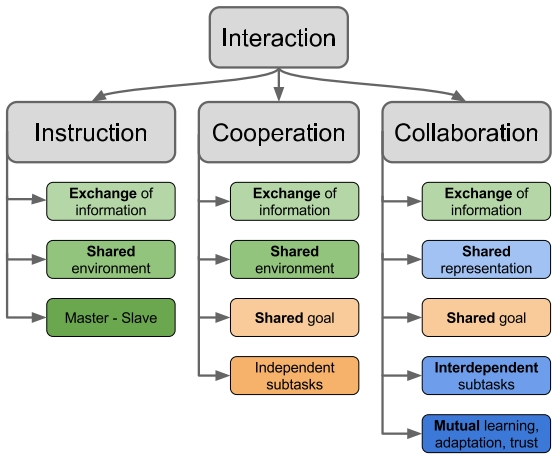
\includegraphics[width=0.75\textwidth]{images/HRC_roles.jpg}
   \caption{Taxonomy of human robot interactions (HRI) \citep{butepage2017human}. Three categories are defined, namely instruction, cooperation and collaboration, based on ascending level of interdependence between the human and the robot partners.}
   \label{pics:butepage2017}
\end{figure}

\begin{description}
\item[Instruction] On the lowest level of interdependence, instruction groups types of interactions, which are a sequence of actions governed by the human. Although there is exchange of information between the two partners and they are sharing an environment, the robot is subordinated to the human in a master-slave paradigm and does not independently try to reach a goal, but merely assists the human in reaching his. A common example is learning from demonstration \citep{argall2009survey}.

\item[Cooperation] This concept is expanded in cooperation tasks to a shared goal, where the goal is divisible in subtasks, on which the partners can work independently. Here, roles are fixed but do not necessarily have to be in a master-slave scenario.

\item[Collaboration] Finally, collaboration groups tasks that require a shared representation of the environment and have subtasks, where the partners are interdependent on each other, i.e., the partners actively engage in the activities of the other. Here, an equal role distribution or role switching between the two is crucial for efficiency and to reduce the cognitive workload for the human.
\end{description}

This project is set within the field of \emph{cooperation}. The goal is to achieve a load sharing algorithm between a robot and a human partner in a cluttered environment. The cooperation comes with several advantages, for both partners. For one, a human physically cooperating with a robotic system can greatly enhance its capabilities and act as a guide or a second control mechanism. In exchange, the robot can take physical load off the human and also reduce the cognitive load, if it is pro-actively 
working towards the shared goal. Finally, the actuation redundancy of any two partners carrying an object, allows for greater flexibility and improved navigation through narrow passages over a single agent carrying the same object \citep{reed2008physical}.

As with any joint carrying task in either human human interaction (HHI) or HRI, the richest sensory exchange channel between the two partners is the haptic feedback through physical coupling of the jointly carried object \citep{reed2006haptic}. Therefore, it is crucial to include the force and torque input from the human into the control loop of the robot. Similarly, a robot which is actively contributing to the shared goal by its obstacle avoidance, although being bound in a fixed subordinate role to the human, will greatly enhance the system.

In the following chapters, we will first analyse other work that has been done in the field of load sharing, then derive the necessary theory for our algorithm before we elaborate on our implementation and finally validate the algorithm in real world scenarios.
